\usetikzlibrary{arrows.meta}
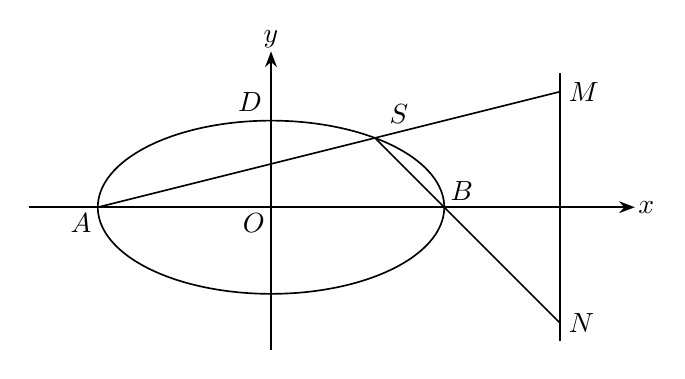
\begin{tikzpicture}[x=1.1cm,y=1.1cm,line width=.6pt,>=Stealth,font=\normalsize]
  \def\ellA{2}
  \def\ellB{1}
  \coordinate (O) at (0,0);
  \coordinate (A) at (-2,0);
  \coordinate (B) at (2,0);
  \coordinate (D) at (0,1);
  \coordinate (S) at (1.2,0.8);
  \coordinate (M) at (3.333333,1.333333);
  \coordinate (N) at (3.333333,-1.333333);
  \draw[->] (-2.8,0) -- (4.2,0) node[right,inner sep=1pt] {$x$};
  \draw[->] (0,-1.65) -- (0,1.8) node[above,inner sep=1pt] {$y$};
  \draw[domain=0:360,samples=201,smooth,variable=\t] plot ({\ellA*cos(\t)},{\ellB*sin(\t)});
  \draw (3.333333,-1.55) -- (3.333333,1.55);
  \draw (A) -- (M);
  \draw (S) -- (N);
  \node[below left,inner sep=2pt] at (O) {$O$};
  \node[below left,inner sep=2pt] at (A) {$A$};
  \node[above right,inner sep=2pt] at (B) {$B$};
  \node[above left,inner sep=3pt] at (D) {$D$};
  \node[above right,inner sep=5pt] at (S) {$S$};
  \node[right,inner sep=3pt] at (M) {$M$};
  \node[right,inner sep=3pt] at (N) {$N$};
\end{tikzpicture}
